\newcommand{\coursemodule}{Module 02}
% ════════════════════════════════════════════════════════════════════════════
% Pixels, Frames & Transformers: shared Beamer preamble (WUR style)
% Adapted from the preamble of Bags, Vectors & Transformers.
%
% Use in a module deck (from <part>/<module>/slides/):
%   \newcommand{\coursemodule}{Module 01}
%   % ════════════════════════════════════════════════════════════════════════════
% Pixels, Frames & Transformers: shared Beamer preamble (WUR style)
% Adapted from the preamble of Bags, Vectors & Transformers.
%
% Use in a module deck (from <part>/<module>/slides/):
%   \newcommand{\coursemodule}{Module 01}
%   % ════════════════════════════════════════════════════════════════════════════
% Pixels, Frames & Transformers: shared Beamer preamble (WUR style)
% Adapted from the preamble of Bags, Vectors & Transformers.
%
% Use in a module deck (from <part>/<module>/slides/):
%   \newcommand{\coursemodule}{Module 01}
%   \input{../../../shared/preamble.tex}
%   \begin{document}
%   \moduletitle{Images as Data}
%   ...
% Compile with: latexmk -pdf <deck>.tex
% ════════════════════════════════════════════════════════════════════════════

\documentclass[aspectratio=169]{beamer}

% ── Packages ────────────────────────────────────────────────────────────────
\usepackage[T1]{fontenc}
\usepackage[utf8]{inputenc}
\usepackage{lmodern}
\usepackage{microtype}
\usepackage{xcolor}
\usepackage{tikz}
\usetikzlibrary{arrows.meta, positioning, calc, shapes.geometric, decorations.pathreplacing, matrix, fit}
\usepackage{booktabs}
\usepackage{fontawesome5}
\usepackage{array}
\usepackage[most]{tcolorbox}

\providecommand{\coursemodule}{}

% ── WUR color palette ───────────────────────────────────────────────────────
\definecolor{wurgreen}{HTML}{34B233}
\definecolor{darkgreen}{HTML}{1F6B1E}
\definecolor{lightgreen}{HTML}{E8F7E8}
\definecolor{darknavy}{HTML}{1A1A2E}
\definecolor{midgray}{HTML}{6B7280}
\definecolor{lightgray}{HTML}{F3F4F6}
\definecolor{bodytext}{HTML}{1F2937}
\definecolor{codegreen}{HTML}{9AE6B4}
\definecolor{warnred}{HTML}{FEE2E2}
\definecolor{warnborder}{HTML}{EF4444}

% ── Beamer theme ────────────────────────────────────────────────────────────
\usetheme{default}
\usecolortheme{default}
\usefonttheme{professionalfonts}
\setbeamertemplate{navigation symbols}{}
\setbeamertemplate{itemize items}{\textcolor{wurgreen}{\textbullet}}
\setbeamertemplate{itemize subitem}{\textcolor{midgray}{--}}
\setbeamertemplate{enumerate items}{\textcolor{wurgreen}{\textbf{\insertenumlabel.}}}
\setbeamercolor{frametitle}{fg=white, bg=darknavy}
\setbeamertemplate{frametitle}{%
  \begin{beamercolorbox}[wd=\paperwidth, ht=1.1cm, dp=0.2cm, leftskip=0.6cm]{frametitle}
    \usebeamerfont{frametitle}\insertframetitle
  \end{beamercolorbox}%
}
\setbeamerfont{frametitle}{size=\large, series=\bfseries}
\setbeamercolor{background canvas}{bg=white}
\setbeamercolor{normal text}{fg=bodytext}
\setbeamerfont{normal text}{size=\small}
\setbeamertemplate{footline}{%
  \begin{beamercolorbox}[wd=\paperwidth, ht=0.4cm, dp=0.15cm]{footline}%
    \hspace{0.5cm}%
    \textcolor{midgray}{\tiny Pixels, Frames \& Transformers · \coursemodule\ · Wageningen University \& Research}%
    \hfill%
    \textcolor{midgray}{\tiny \insertframenumber}%
    \hspace{0.4cm}%
  \end{beamercolorbox}%
}

% ── Boxes ───────────────────────────────────────────────────────────────────
\tcbset{wurbase/.style={arc=3pt, boxrule=0.6pt, left=7pt, right=7pt, top=5pt, bottom=5pt,
                        fontupper=\small, before skip=4pt, after skip=4pt}}
\newtcolorbox{greenbox}[1][]{wurbase, colback=lightgreen, colframe=wurgreen, #1}
\newtcolorbox{graybox}[1][]{wurbase, colback=lightgray, colframe=lightgray, #1}
\newtcolorbox{navybox}[1][]{wurbase, colback=darknavy, colframe=darknavy, colupper=white, #1}
\newtcolorbox{warnbox}[1][]{wurbase, colback=warnred, colframe=warnborder, #1}
\newtcolorbox{codebox}[1][]{wurbase, colback=darknavy, colframe=darknavy, colupper=white,
                            fontupper=\ttfamily\scriptsize, left=6pt, top=4pt, bottom=4pt, #1}

% ── Title slide ─────────────────────────────────────────────────────────────
\newcommand{\moduletitle}[1]{%
{
\setbeamertemplate{footline}{}
\begin{frame}[plain]
  \begin{tikzpicture}[remember picture, overlay]
    \fill[darknavy] (current page.south west) rectangle (current page.north east);
    \fill[wurgreen] (current page.south west) rectangle ([xshift=0.45cm]current page.north west);
    \node[anchor=west, text=white, font=\huge\bfseries, text width=13cm]
      at ([xshift=1.1cm, yshift=1.2cm]current page.west) {Pixels, Frames \& Transformers};
    \node[anchor=west, text=wurgreen, font=\large, text width=13cm]
      at ([xshift=1.1cm, yshift=0.05cm]current page.west) {#1 · \coursemodule};
    \node[anchor=west, text=midgray, font=\small, text width=12cm]
      at ([xshift=1.1cm, yshift=-1.5cm]current page.west)
      {Denise J. Roth, PhD Candidate\\
       Strategic Communication Group · Wageningen University \& Research};
  \end{tikzpicture}
\end{frame}
}}

% ── Small helpers ───────────────────────────────────────────────────────────
\newcommand{\keyterm}[1]{\textbf{\textcolor{darkgreen}{#1}}}
\newcommand{\muted}[1]{\textcolor{midgray}{#1}}
\newcommand{\credit}[1]{{\tiny\textcolor{midgray}{#1}}}
\newcommand{\notebookslide}[1]{%
\begin{frame}{In the Notebook}
\vspace{0.1cm}
#1
\end{frame}}
\newcommand{\nbitem}[2]{\item[\textcolor{wurgreen}{#1}] #2}

%   \begin{document}
%   \moduletitle{Images as Data}
%   ...
% Compile with: latexmk -pdf <deck>.tex
% ════════════════════════════════════════════════════════════════════════════

\documentclass[aspectratio=169]{beamer}

% ── Packages ────────────────────────────────────────────────────────────────
\usepackage[T1]{fontenc}
\usepackage[utf8]{inputenc}
\usepackage{lmodern}
\usepackage{microtype}
\usepackage{xcolor}
\usepackage{tikz}
\usetikzlibrary{arrows.meta, positioning, calc, shapes.geometric, decorations.pathreplacing, matrix, fit}
\usepackage{booktabs}
\usepackage{fontawesome5}
\usepackage{array}
\usepackage[most]{tcolorbox}

\providecommand{\coursemodule}{}

% ── WUR color palette ───────────────────────────────────────────────────────
\definecolor{wurgreen}{HTML}{34B233}
\definecolor{darkgreen}{HTML}{1F6B1E}
\definecolor{lightgreen}{HTML}{E8F7E8}
\definecolor{darknavy}{HTML}{1A1A2E}
\definecolor{midgray}{HTML}{6B7280}
\definecolor{lightgray}{HTML}{F3F4F6}
\definecolor{bodytext}{HTML}{1F2937}
\definecolor{codegreen}{HTML}{9AE6B4}
\definecolor{warnred}{HTML}{FEE2E2}
\definecolor{warnborder}{HTML}{EF4444}

% ── Beamer theme ────────────────────────────────────────────────────────────
\usetheme{default}
\usecolortheme{default}
\usefonttheme{professionalfonts}
\setbeamertemplate{navigation symbols}{}
\setbeamertemplate{itemize items}{\textcolor{wurgreen}{\textbullet}}
\setbeamertemplate{itemize subitem}{\textcolor{midgray}{--}}
\setbeamertemplate{enumerate items}{\textcolor{wurgreen}{\textbf{\insertenumlabel.}}}
\setbeamercolor{frametitle}{fg=white, bg=darknavy}
\setbeamertemplate{frametitle}{%
  \begin{beamercolorbox}[wd=\paperwidth, ht=1.1cm, dp=0.2cm, leftskip=0.6cm]{frametitle}
    \usebeamerfont{frametitle}\insertframetitle
  \end{beamercolorbox}%
}
\setbeamerfont{frametitle}{size=\large, series=\bfseries}
\setbeamercolor{background canvas}{bg=white}
\setbeamercolor{normal text}{fg=bodytext}
\setbeamerfont{normal text}{size=\small}
\setbeamertemplate{footline}{%
  \begin{beamercolorbox}[wd=\paperwidth, ht=0.4cm, dp=0.15cm]{footline}%
    \hspace{0.5cm}%
    \textcolor{midgray}{\tiny Pixels, Frames \& Transformers · \coursemodule\ · Wageningen University \& Research}%
    \hfill%
    \textcolor{midgray}{\tiny \insertframenumber}%
    \hspace{0.4cm}%
  \end{beamercolorbox}%
}

% ── Boxes ───────────────────────────────────────────────────────────────────
\tcbset{wurbase/.style={arc=3pt, boxrule=0.6pt, left=7pt, right=7pt, top=5pt, bottom=5pt,
                        fontupper=\small, before skip=4pt, after skip=4pt}}
\newtcolorbox{greenbox}[1][]{wurbase, colback=lightgreen, colframe=wurgreen, #1}
\newtcolorbox{graybox}[1][]{wurbase, colback=lightgray, colframe=lightgray, #1}
\newtcolorbox{navybox}[1][]{wurbase, colback=darknavy, colframe=darknavy, colupper=white, #1}
\newtcolorbox{warnbox}[1][]{wurbase, colback=warnred, colframe=warnborder, #1}
\newtcolorbox{codebox}[1][]{wurbase, colback=darknavy, colframe=darknavy, colupper=white,
                            fontupper=\ttfamily\scriptsize, left=6pt, top=4pt, bottom=4pt, #1}

% ── Title slide ─────────────────────────────────────────────────────────────
\newcommand{\moduletitle}[1]{%
{
\setbeamertemplate{footline}{}
\begin{frame}[plain]
  \begin{tikzpicture}[remember picture, overlay]
    \fill[darknavy] (current page.south west) rectangle (current page.north east);
    \fill[wurgreen] (current page.south west) rectangle ([xshift=0.45cm]current page.north west);
    \node[anchor=west, text=white, font=\huge\bfseries, text width=13cm]
      at ([xshift=1.1cm, yshift=1.2cm]current page.west) {Pixels, Frames \& Transformers};
    \node[anchor=west, text=wurgreen, font=\large, text width=13cm]
      at ([xshift=1.1cm, yshift=0.05cm]current page.west) {#1 · \coursemodule};
    \node[anchor=west, text=midgray, font=\small, text width=12cm]
      at ([xshift=1.1cm, yshift=-1.5cm]current page.west)
      {Denise J. Roth, PhD Candidate\\
       Strategic Communication Group · Wageningen University \& Research};
  \end{tikzpicture}
\end{frame}
}}

% ── Small helpers ───────────────────────────────────────────────────────────
\newcommand{\keyterm}[1]{\textbf{\textcolor{darkgreen}{#1}}}
\newcommand{\muted}[1]{\textcolor{midgray}{#1}}
\newcommand{\credit}[1]{{\tiny\textcolor{midgray}{#1}}}
\newcommand{\notebookslide}[1]{%
\begin{frame}{In the Notebook}
\vspace{0.1cm}
#1
\end{frame}}
\newcommand{\nbitem}[2]{\item[\textcolor{wurgreen}{#1}] #2}

%   \begin{document}
%   \moduletitle{Images as Data}
%   ...
% Compile with: latexmk -pdf <deck>.tex
% ════════════════════════════════════════════════════════════════════════════

\documentclass[aspectratio=169]{beamer}

% ── Packages ────────────────────────────────────────────────────────────────
\usepackage[T1]{fontenc}
\usepackage[utf8]{inputenc}
\usepackage{lmodern}
\usepackage{microtype}
\usepackage{xcolor}
\usepackage{tikz}
\usetikzlibrary{arrows.meta, positioning, calc, shapes.geometric, decorations.pathreplacing, matrix, fit}
\usepackage{booktabs}
\usepackage{fontawesome5}
\usepackage{array}
\usepackage[most]{tcolorbox}

\providecommand{\coursemodule}{}

% ── WUR color palette ───────────────────────────────────────────────────────
\definecolor{wurgreen}{HTML}{34B233}
\definecolor{darkgreen}{HTML}{1F6B1E}
\definecolor{lightgreen}{HTML}{E8F7E8}
\definecolor{darknavy}{HTML}{1A1A2E}
\definecolor{midgray}{HTML}{6B7280}
\definecolor{lightgray}{HTML}{F3F4F6}
\definecolor{bodytext}{HTML}{1F2937}
\definecolor{codegreen}{HTML}{9AE6B4}
\definecolor{warnred}{HTML}{FEE2E2}
\definecolor{warnborder}{HTML}{EF4444}

% ── Beamer theme ────────────────────────────────────────────────────────────
\usetheme{default}
\usecolortheme{default}
\usefonttheme{professionalfonts}
\setbeamertemplate{navigation symbols}{}
\setbeamertemplate{itemize items}{\textcolor{wurgreen}{\textbullet}}
\setbeamertemplate{itemize subitem}{\textcolor{midgray}{--}}
\setbeamertemplate{enumerate items}{\textcolor{wurgreen}{\textbf{\insertenumlabel.}}}
\setbeamercolor{frametitle}{fg=white, bg=darknavy}
\setbeamertemplate{frametitle}{%
  \begin{beamercolorbox}[wd=\paperwidth, ht=1.1cm, dp=0.2cm, leftskip=0.6cm]{frametitle}
    \usebeamerfont{frametitle}\insertframetitle
  \end{beamercolorbox}%
}
\setbeamerfont{frametitle}{size=\large, series=\bfseries}
\setbeamercolor{background canvas}{bg=white}
\setbeamercolor{normal text}{fg=bodytext}
\setbeamerfont{normal text}{size=\small}
\setbeamertemplate{footline}{%
  \begin{beamercolorbox}[wd=\paperwidth, ht=0.4cm, dp=0.15cm]{footline}%
    \hspace{0.5cm}%
    \textcolor{midgray}{\tiny Pixels, Frames \& Transformers · \coursemodule\ · Wageningen University \& Research}%
    \hfill%
    \textcolor{midgray}{\tiny \insertframenumber}%
    \hspace{0.4cm}%
  \end{beamercolorbox}%
}

% ── Boxes ───────────────────────────────────────────────────────────────────
\tcbset{wurbase/.style={arc=3pt, boxrule=0.6pt, left=7pt, right=7pt, top=5pt, bottom=5pt,
                        fontupper=\small, before skip=4pt, after skip=4pt}}
\newtcolorbox{greenbox}[1][]{wurbase, colback=lightgreen, colframe=wurgreen, #1}
\newtcolorbox{graybox}[1][]{wurbase, colback=lightgray, colframe=lightgray, #1}
\newtcolorbox{navybox}[1][]{wurbase, colback=darknavy, colframe=darknavy, colupper=white, #1}
\newtcolorbox{warnbox}[1][]{wurbase, colback=warnred, colframe=warnborder, #1}
\newtcolorbox{codebox}[1][]{wurbase, colback=darknavy, colframe=darknavy, colupper=white,
                            fontupper=\ttfamily\scriptsize, left=6pt, top=4pt, bottom=4pt, #1}

% ── Title slide ─────────────────────────────────────────────────────────────
\newcommand{\moduletitle}[1]{%
{
\setbeamertemplate{footline}{}
\begin{frame}[plain]
  \begin{tikzpicture}[remember picture, overlay]
    \fill[darknavy] (current page.south west) rectangle (current page.north east);
    \fill[wurgreen] (current page.south west) rectangle ([xshift=0.45cm]current page.north west);
    \node[anchor=west, text=white, font=\huge\bfseries, text width=13cm]
      at ([xshift=1.1cm, yshift=1.2cm]current page.west) {Pixels, Frames \& Transformers};
    \node[anchor=west, text=wurgreen, font=\large, text width=13cm]
      at ([xshift=1.1cm, yshift=0.05cm]current page.west) {#1 · \coursemodule};
    \node[anchor=west, text=midgray, font=\small, text width=12cm]
      at ([xshift=1.1cm, yshift=-1.5cm]current page.west)
      {Denise J. Roth, PhD Candidate\\
       Strategic Communication Group · Wageningen University \& Research};
  \end{tikzpicture}
\end{frame}
}}

% ── Small helpers ───────────────────────────────────────────────────────────
\newcommand{\keyterm}[1]{\textbf{\textcolor{darkgreen}{#1}}}
\newcommand{\muted}[1]{\textcolor{midgray}{#1}}
\newcommand{\credit}[1]{{\tiny\textcolor{midgray}{#1}}}
\newcommand{\notebookslide}[1]{%
\begin{frame}{In the Notebook}
\vspace{0.1cm}
#1
\end{frame}}
\newcommand{\nbitem}[2]{\item[\textcolor{wurgreen}{#1}] #2}


\begin{document}

\moduletitle{Building an Image Corpus}

% ─────────────────────────────────────────────────────────────────────────────
\begin{frame}{Collection Comes First}
Images are easy to find and hard to use properly. Four questions decide what you can do with a
corpus once you have it, so answer them \textbf{before} the first download:

\vspace{0.2cm}
\begin{columns}[T]
\begin{column}{0.48\textwidth}
\begin{greenbox}
\textbf{\faBalanceScale\ Rights}\\
Who holds the copyright, and under which license can I use the images?
\end{greenbox}
\begin{greenbox}
\textbf{\faGlobeEurope\ Platforms}\\
What do the terms of the site or archive allow: automated access, research use?
\end{greenbox}
\end{column}
\begin{column}{0.48\textwidth}
\begin{greenbox}
\textbf{\faUsers\ People}\\
Do the images show identifiable people? What is my legal basis, and how do I protect them?
\end{greenbox}
\begin{greenbox}
\textbf{\faDatabase\ Sharing}\\
What will I need to publish (figures, data, a replication package), and am I allowed to?
\end{greenbox}
\end{column}
\end{columns}
\end{frame}

% ─────────────────────────────────────────────────────────────────────────────
\begin{frame}{Where Research Images Come From}
\vspace{0.1cm}
{\footnotesize
\begin{tabular}{@{}>{\raggedright\arraybackslash}p{2.9cm}>{\raggedright\arraybackslash}p{5.4cm}>{\raggedright\arraybackslash}p{5.0cm}@{}}
\toprule
\textbf{Source} & \textbf{What you get} & \textbf{Typical constraints} \\
\midrule
Archives and museums & curated collections with rich metadata, increasingly openly licensed & reuse terms vary per collection \\[2pt]
Wikimedia Commons & freely licensed images, each with author and license & categories are volunteer-made and messy \\[2pt]
Open data projects & e.g.\ Open Food Facts, government photo collections & usually open licenses with attribution \\[2pt]
Platform research access & YouTube Data API, TikTok Research API, Meta Content Library, the EU Digital Services Act (Art.~40) & approval needed; mostly \textbf{metadata}, not the media files \\[2pt]
Data donation & participants share their own data with you & their consent doesn't cover others in their photos \\[2pt]
Scraping websites & whatever is publicly visible & copyright, terms of service and privacy all apply \\
\bottomrule
\end{tabular}}

\vspace{0.15cm}
\muted{This module uses two sources that are open by design. The habits carry over to the harder
ones, where they matter even more.}
\end{frame}

% ─────────────────────────────────────────────────────────────────────────────
\newcommand{\yes}{\textcolor{wurgreen}{\faCheck}}
\newcommand{\no}{\textcolor{warnborder}{\faTimes}}
\newcommand{\maybe}{\textcolor{midgray}{\textbf{?}}}
\begin{frame}{Licenses in Practice}
\vspace{0.1cm}
{\footnotesize
\begin{tabular}{@{}l>{\centering\arraybackslash}p{1.1cm}>{\centering\arraybackslash}p{1.5cm}>{\centering\arraybackslash}p{1.1cm}>{\raggedright\arraybackslash}p{6.0cm}@{}}
\toprule
\textbf{License} & \textbf{Analyze} & \textbf{Show in a paper} & \textbf{Share files} & \textbf{Conditions} \\
\midrule
Public domain, CC0 & \yes & \yes & \yes & none (credit the source anyway) \\
CC BY & \yes & \yes & \yes & credit the creator, link the license, note changes \\
CC BY-SA & \yes & \yes & \yes & as BY; anything built from it keeps the license \\
CC BY-NC & \yes & \maybe & \yes & non-commercial only; check your publisher \\
CC BY-ND & \yes & \yes & \yes & no adaptations (cropping can count as one) \\
All rights reserved & \maybe & \maybe & \no & research exceptions; quotation rules \\
\bottomrule
\end{tabular}}

\vspace{0.15cm}
\begin{graybox}
\textbf{EU research exception.} Article 3 of the Copyright in the Digital Single Market Directive
(2019/790) lets research organizations mine works they can lawfully access, images included.
That covers \emph{analyzing} them, not redistributing them.
\end{graybox}
\credit{A starting point, not legal advice. Your research data office can help with specific cases.}
\end{frame}

% ─────────────────────────────────────────────────────────────────────────────
\begin{frame}{Can I Use This Image in My Research?}
\centering
\begin{tikzpicture}[
  node distance=0.5cm,
  q/.style={draw=darknavy, fill=darknavy, text=white, rounded corners=3pt, align=center,
            font=\footnotesize\bfseries, inner sep=5pt, text width=3.0cm},
  a/.style={draw=wurgreen, fill=lightgreen, rounded corners=3pt, align=left,
            font=\footnotesize, inner sep=5pt, text width=5.6cm},
  stop/.style={draw=warnborder, fill=warnred, rounded corners=3pt, align=left,
            font=\footnotesize, inner sep=5pt, text width=3.0cm},
  s/.style={draw=midgray, fill=lightgray, rounded corners=3pt, align=center,
            font=\footnotesize, inner sep=5pt, text width=2.3cm},
  arr/.style={-{Stealth[length=2mm]}, thick, color=midgray},
  lab/.style={font=\scriptsize\bfseries, color=midgray}]
\node[s] (start) {An image you want to use};
\node[q, right=0.7cm of start] (q1) {Public domain or an open license?};
\node[a, right=1.0cm of q1] (a1) {\textbf{Analyze, show and share it}, following the license:
credit (BY), same license (SA), non-commercial (NC), no changes (ND)};
\node[q, below=0.9cm of q1] (q2) {Lawful access, at a research organization?};
\node[a, right=1.0cm of q2] (a2) {\textbf{Analyze it} under the research exception.
Show it only under quotation rules. \textbf{Share identifiers and code}, not the files.};
\node[stop, left=0.7cm of q2] (a3) {Ask the rights holder, or find another source.};
\draw[arr] (start) -- (q1);
\draw[arr] (q1) -- node[lab, above] {yes} (a1);
\draw[arr] (q1) -- node[lab, right] {no} (q2);
\draw[arr] (q2) -- node[lab, above] {yes} (a2);
\draw[arr] (q2) -- node[lab, above] {no} (a3);
\end{tikzpicture}

\vspace{0.3cm}
\begin{warnbox}
\textbf{\faUsers\ Whatever the license:} if the image shows identifiable people, it is
\textbf{personal data} under the GDPR. You need a legal basis, should collect only what you need,
store it securely, and think twice about what you publish.
\end{warnbox}
\credit{EU perspective; rules differ elsewhere. A starting point, not legal advice: ask your data steward or privacy officer.}
\end{frame}

% ─────────────────────────────────────────────────────────────────────────────
\begin{frame}{People in Pictures}
\begin{columns}[T]
\begin{column}{0.48\textwidth}
\begin{warnbox}
\textbf{\faUserShield\ Faces are personal data}\\
A photo of an identifiable person is personal data, even if you don't know their name.
Research is allowed, with safeguards.
\end{warnbox}
\begin{warnbox}
\textbf{\faFingerprint\ Recognition is biometric}\\
Using a face to \emph{identify} someone makes it biometric data, a special category with stricter
rules. Analyzing a photo without identifying anyone is not.
\end{warnbox}
\end{column}
\begin{column}{0.48\textwidth}
\begin{warnbox}
\textbf{\faUserTie\ Public role or bystander?}\\
A politician at work is not a protester in a crowd, who may not want their participation known.
\end{warnbox}
\begin{warnbox}
\textbf{\faChild\ Minors and what you publish}\\
Children need extra protection. Figures reach far more people than your analysis does: blurring
faces is often wise.
\end{warnbox}
\end{column}
\end{columns}
\muted{Talk to your privacy officer and ethics committee before you collect images of people.}
\end{frame}

% ─────────────────────────────────────────────────────────────────────────────
\begin{frame}{Download Politely, Keep a Manifest}
\begin{columns}[T]
\begin{column}{0.40\textwidth}
\textbf{Polite collection}
\begin{itemize}
\item \keyterm{Identify yourself} with a User-Agent: project name and contact
\item \keyterm{Pause} between requests and respect stated limits
\item \keyterm{Never download twice}: skip what you have
\item \keyterm{Record failures} instead of crashing
\item Thumbnails are often enough
\end{itemize}
\end{column}
\begin{column}{0.57\textwidth}
\textbf{A manifest: one row per image}

\vspace{0.1cm}
{\footnotesize
\begin{tabular}{@{}lp{5.2cm}@{}}
\toprule
\texttt{local\_path} & where the file is on your disk \\
\texttt{source}, \texttt{page\_url} & where it came from \\
\texttt{license}, \texttt{author} & what you may do with it, and whom to credit \\
\texttt{downloaded\_at} & when you got it \\
\texttt{sha256} & a checksum: proof the file hasn't changed \\
\bottomrule
\end{tabular}}

\vspace{0.2cm}
\begin{greenbox}
Every analysis starts by reading the manifest, not by listing a folder. It is the single most
useful thing you can keep about a corpus.
\end{greenbox}
\end{column}
\end{columns}
\end{frame}

% ─────────────────────────────────────────────────────────────────────────────
\begin{frame}{Exact and Near Duplicates}
\centering
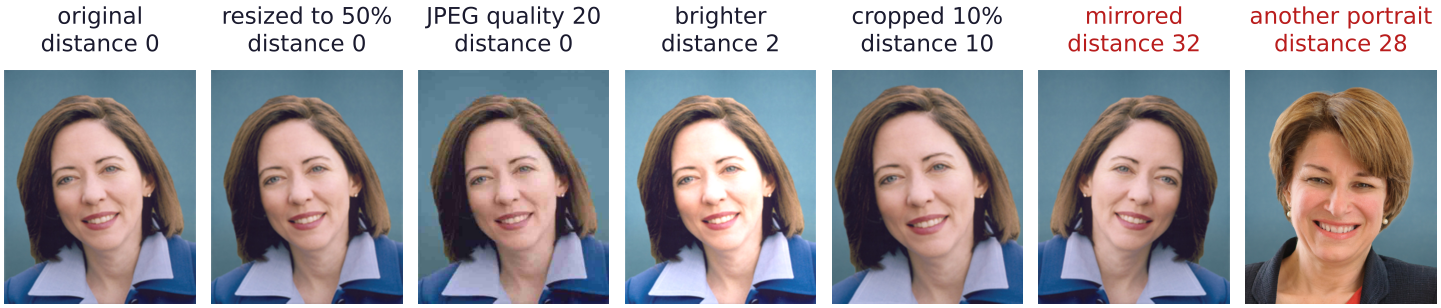
\includegraphics[width=0.8\textwidth]{figures/phash_variants.png}\\
\credit{Official portraits of Sen.\ Maria Cantwell and Sen.\ Amy Klobuchar, public domain, via unitedstates/images.}

\raggedright
\begin{columns}[T]
\begin{column}{0.48\textwidth}
\begin{graybox}
\textbf{Checksum (SHA-256)}\\
changes completely if one bit changes, so it finds only \textbf{identical files}. None of
these variants shares the original's.
\end{graybox}
\end{column}
\begin{column}{0.48\textwidth}
\begin{greenbox}
\textbf{Perceptual hash}\\
64 bits that summarize a tiny grayscale copy. Distance = bits that differ (0--64). Around
\textbf{10} catches resized and recompressed copies.
\end{greenbox}
\end{column}
\end{columns}
\muted{Duplicates inflate counts and can land in both training and test data, making a classifier
look better than it is.}
\end{frame}

% ─────────────────────────────────────────────────────────────────────────────
\begin{frame}{Share What You Can, Document Everything}
\begin{columns}[T]
\begin{column}{0.46\textwidth}
\textbf{You can almost always share}
\begin{itemize}
\item the \keyterm{manifest}: identifiers, URLs, licenses, authors, dates, checksums
\item your \keyterm{code} for collecting, filtering and deduplicating
\item \keyterm{derived data}: features, embeddings, codes and labels
\end{itemize}
\vspace{0.1cm}
\muted{With these, others can rebuild your corpus even when the images themselves can't be
redistributed.}
\end{column}
\begin{column}{0.5\textwidth}
\begin{navybox}
\textbf{A datasheet} \textcolor{codegreen}{(Gebru et al., 2021)}\\[3pt]
\textbf{Motivation:} why was the corpus made?\\
\textbf{Composition:} what is in it, from when and where?\\
\textbf{Collection:} how were images selected, and what was left out?\\
\textbf{Gaps and biases:} who and what is missing?\\
\textbf{Uses:} what should it \emph{not} be used for?
\end{navybox}
\muted{Half an hour of writing that saves your future self, and your reviewers, much more.}
\end{column}
\end{columns}
\end{frame}

% ─────────────────────────────────────────────────────────────────────────────
\notebookslide{
\begin{itemize}
\setlength{\itemsep}{5pt}
\nbitem{\faBalanceScale}{Four scenarios: licenses, people and publishing}
\nbitem{\faWikipediaW}{The Wikimedia Commons API: protest photos with license and author}
\nbitem{\faDownload}{Polite downloading and a manifest with checksums}
\nbitem{\faUtensils}{Breakfast cereal packaging from Open Food Facts}
\nbitem{\faCopy}{Exact duplicates with checksums, near duplicates with perceptual hashes}
\nbitem{\faClipboardList}{A datasheet for your corpus}
\end{itemize}

\vspace{0.35cm}
\muted{\footnotesize part1\_pixels/02\_building\_an\_image\_corpus/notebooks/\\
02\_building\_an\_image\_corpus\_exercises.ipynb · 7 exercises · CPU runtime · about 10 minutes of
downloads}
}

\end{document}
